%! app: Decidable Languages, Undecidable Languages
%! outcome: Formal definition of automata, Informal definition of automata, Classify language, Find example languages

We are ready to introduce a formal model that will capture a notion of general purpose computation.
\begin{itemize}
\item {\it Similar to DFA, NFA, PDA}: input will be an arbitrary string over a fixed alphabet.
\item {\it Different from NFA, PDA}: machine is deterministic.
\item {\it Different from DFA, NFA, PDA}: read-write head can move both to the left and to the right,
and can extend to the right past the original input.
\item {\it Similar to DFA, NFA, PDA}: transition function drives computation one step at a time 
by moving within a finite set of states, always starting at designated start state.
\item {\it Different from DFA, NFA, PDA}: the special states for rejecting and accepting take effect immediately.
\end{itemize}

\vspace{-10pt}

(See more details: Sipser p. 166)

\vfill

Formally: a  Turing machine is $M= (Q, \Sigma, \Gamma, \delta, q_0, q_{accept}, q_{reject})$ 
where $\delta$ is the {\bf transition function} 
\[
  \delta: Q\times \Gamma \to Q \times \Gamma \times \{L, R\}
\]
The {\bf computation} of $M$ on a string $w$ over $\Sigma$  is:

\vspace{-10pt}

\begin{itemize}
\setlength{\itemsep}{0pt}
\item Read/write head starts at leftmost position on tape. 
\item Input string is written on $|w|$-many leftmost cells of tape, 
rest of  the tape cells have  the blank symbol. {\bf Tape alphabet} 
is $\Gamma$ with $\textvisiblespace\in \Gamma$ and $\Sigma \subseteq \Gamma$.
The blank symbol $\textvisiblespace \notin \Sigma$.
\item Given current state of machine and current symbol being read at the tape head, 
the machine transitions to next state, writes a symbol to the current position  of the 
tape  head (overwriting existing symbol), and moves the tape head L or R (if possible). 
\item Computation ends {\bf if and when} machine enters either the accept or the reject state.
This is called {\bf halting}.
Note: $q_{accept} \neq q_{reject}$.
\end{itemize}

The {\bf language recognized by the  Turing machine} $M$,  is  $L(M) = \{ w \in \Sigma^* \mid w \textrm{ is accepted by } M\}$,
which is defined as
\[
  \{ w \in \Sigma^* \mid \textrm{computation of $M$ on $w$ halts after entering the accept state}\}
\]




\newpage
\begin{multicols}{2}
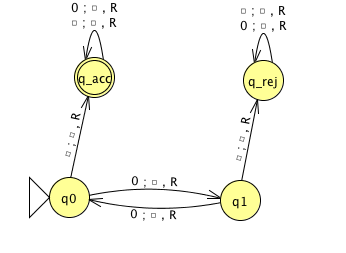
\includegraphics[width=2.5in]{../../resources/machines/Lect13TM1.png}

\columnbreak
Formal definition:

\vspace{10pt}

Sample computation: 

\begin{tabular}{|c|c|c|c|c|c|c|}
\hline
\multicolumn{1}{|c}{$q0\downarrow$} &  \multicolumn{6}{c|}{\phantom{A}}\\
\hline
$0$ & $0$  & $0$ & $\textvisiblespace $& $\textvisiblespace $& $\textvisiblespace $&  $\textvisiblespace $\\
\hline
\multicolumn{7}{|c|}{\phantom{A}}\\
\hline
\phantom{AA} & \phantom{AA}& \phantom{AA}& \phantom{AA}& \phantom{AA}& \phantom{AA}& \phantom{AA} \\
\hline
\multicolumn{7}{|c|}{\phantom{A}}\\
\hline
\phantom{AA} & \phantom{AA}& \phantom{AA}& \phantom{AA}& \phantom{AA}& \phantom{AA}& \phantom{AA} \\
\hline
\multicolumn{7}{|c|}{\phantom{A}}\\
\hline
\phantom{AA} & \phantom{AA}& \phantom{AA}& \phantom{AA}& \phantom{AA}& \phantom{AA}& \phantom{AA} \\
\hline
\multicolumn{7}{|c|}{\phantom{A}}\\
\hline
\phantom{AA} & \phantom{AA}& \phantom{AA}& \phantom{AA}& \phantom{AA}& \phantom{AA}& \phantom{AA} \\
\hline
\end{tabular}
\end{multicols}
\vfill

The language recognized by this machine is \ldots

\vfill
 

{\bf Describing  Turing machines} (Sipser p. 185) To define a Turing machine, we could give a 
\begin{itemize}
\item {\bf Formal definition}: the $7$-tuple of parameters including set of states, 
input alphabet, tape alphabet, transition function, start state, accept state, and reject state; or,
\item {\bf Implementation-level definition}: English prose that describes the Turing machine head 
movements relative to contents of tape, and conditions for accepting / rejecting based on those contents.
\item {\bf High-level description}: description of algorithm (precise sequence of instructions), 
without implementation details of machine. As part of this description, can ``call" and run 
another TM as a subroutine.
\end{itemize}
  
\newpage
Fix $\Sigma = \{0,1\}$, $\Gamma = \{ 0, 1, \textvisiblespace\}$ for the Turing machines with  the following state diagrams:
  
\begin{center}
  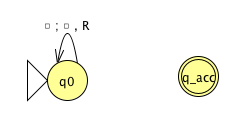
\includegraphics[width=2in]{../../resources/machines/Lect14TM1.png}
\end{center}

Example of string accepted: \\
Example of string rejected: \\


Implementation-level description

\vfill

High-level description

\vfill

\begin{center}
  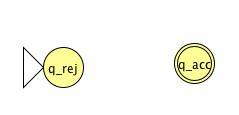
\includegraphics[width=2in]{../../resources/machines/Lect14TM2.png}
\end{center}

Example of string accepted: \\
Example of string rejected: \\


Implementation-level description

\vfill

High-level description

\vfill

\newpage
\begin{center}
  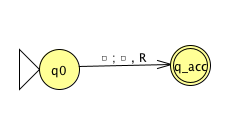
\includegraphics[width=2in]{../../resources/machines/Lect14TM3.png}
\end{center}

Example of string accepted: \\
Example of string rejected: \\


Implementation-level description

\vfill

High-level description

\vfill

\begin{center}
  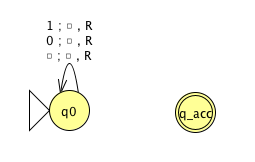
\includegraphics[width=2in]{../../resources/machines/Lect14TM4.png}
\end{center}

Example of string accepted: \\
Example of string rejected: \\


Implementation-level description

\vfill

High-level description

\vfill

\newpage
